\section{Data}\label{sec:data}

\subsection{Data sources}
We collect air pollution levels using 1600 air quality stations measuring ground-level PM2.5 concentrations from January 2019 to September 2020 as our target variable. To predict PM2.5 concentrations, we extract weekly averaged time-series values for AOD, NO$_2$, Land Use, and Precipitation satellite data from Google Earth Engine. To extract data from the Google Earth Engine\footnote{\url{https://earthengine.google.com}}, we import data from 1st January 2019 to 11th September 2020 from the following satellites:
%
\begin{itemize}
    \item Sentinel-5P NRTI NO$_2$: Near Real-Time Nitrogen Dioxide (NO$_2$),
    \item MCD19A2.006: Terra \& Aqua MAIAC Land Aerosol Optical Depth Daily 1km (AOD),
    \item GPWv411: Population Density Gridded Population of the World (Population Density),
    \item GSMaP Operational: Global Satellite Mapping of Precipitation (Precipitation).
\end{itemize}

\subsection{Data Processing}
The satellites collect data at different temporal and spatial granularities (Table~\ref{tab:datatable}). To standardize the satellite data, we aggregate the satellite data by weekly average (Figure~\ref{fig:2step}). To generate these statistics, we generated a VRT driver (a format driver for GDAL that allows a virtual GDAL dataset to be composed from the other GDAL datasets) to process the data faster.

\begin{table*}[t]
\centering
    \begin{tabular}{lllll}
    \hline
\parbox[t]{2cm}{{\bf Data\\name}} &
\parbox[t]{3cm}{{\bf Data\\type}} &
\parbox[t]{4cm}{{\bf Spatial\\resolution}} &
\parbox[t]{2cm}{{\bf Temporal\\resolution}} &
\parbox[t]{4cm}{{\bf Description}}\\\hline
\parbox[t]{2cm}{PM2.5} &
\parbox[t]{3cm}{Ground Sensor} &
\parbox[t]{3cm}{Point location\\(latitude/longitude)} &
\parbox[t]{2cm}{Hourly} &
\parbox[t]{4cm}{Weekly averaged PM2.5 collected by ground station, source: OpenAQ\footnote{\url{https://openaq.org}}}\\
    Oxford Covid19 Data        &
    Tabular       & 
    National (192 countries)                & 
    Daily               & 
    Lockdown information\\
    Precipitation              &
    Raster        &
    0.1 arc degrees                         &
    Daily               &
    Snapshot of hourly precipitation rate (source: GSMaP Operational: Global Satellite Mapping of Precipitation)\\
    AOD                        &
    Raster        &
    1000 meters                             &
    Daily               &
    Blue band (0.47 $\mu$m) aerosol optical depth over land (Source: MCD19A2.006: Terra \& Aqua MAIAC Land Aerosol Optical Depth)\\
    NO2                        &
    Raster        &
    0.01 arc degrees                        &
    Daily               &
    Total vertical column of NO2 = ratio of NO2 slant column density and total air mass factor). Source: Sentinel-5P NRTI NO2: Near Real-Time Nitrogen Dioxide\\
    Population Density         &
    Raster        & 30 arc seconds                          & Daily               &
    The estimated number of persons per square kilometer. Source: GPWv411: Population Density (Gridded Population of the World Version 4.11)                   \\
    Average Population Density & Tabular       & National                                & Yearly              & ~\\
    Sensor Latitude            & Tabular       & 10m                                     & N/A                 & ~\\
    Sensor Longitude           & Tabular       & 10m                                     & N/A                 & ~\\\hline
    \end{tabular}
    \caption{Details on the datasets used.}
    \label{tab:datatable}
\end{table*}

\begin{figure}[t]
    \centering
    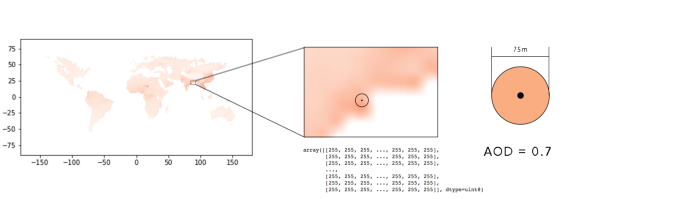
\includegraphics[width=\linewidth]{2step1.png}
    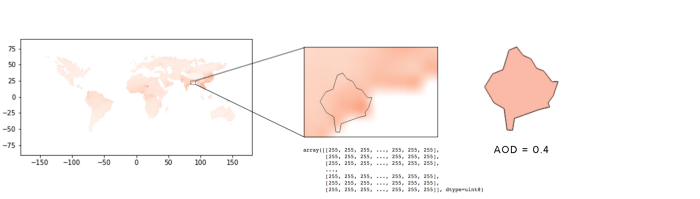
\includegraphics[width=\linewidth]{2step2.png}
    \caption{Panel (a) illustrates the ``local” extraction of AOD from a 75m buffer around a point. Panel (b) illustrates the “city-level” extraction of AOD for each city globally. AOD = Aerosol Optical Depth is a well-known proxy for PM2.5 \cite{Kumar}.
}
    \label{fig:2step}
\end{figure}

Using the VRT file, we extracted weekly averaged data for each of the cities using their geometric shapes. We utilize GADM Shapefiles for this purpose to mask the images and obtain weekly satellite variable averages for city shapes. We extracted weekly averaged data at two different geographic levels, at the local and city-wide levels. At the local level, we extract weekly averaged satellite data values using a local mask defined as a 75m buffer around a ground sensor location. We extract city-wide weekly averaged satellite data values using corresponding city masks from GADM city polygons\footnote{\url{https://gadm.org/data.html}}. In addition to incorporating satellite data as features in the machine learning model, we include several secondary data sources, such as the Covid-19 ``Stringency index" across different spatial and temporal resolutions. See Table 1 for details on the data sources.

Furthermore, we preprocess the PM2.5 station data to ensure we had a reliable training dataset. To do so, we removed PM2.5 values above and equal to 3000 and values below 0. We resampled the PM2.5 values on a weekly basis (Monday Start Day) and use the mean. Using the 75m buffer and the city-wide polygons, we averaged the weekly PM2.5 value for a 75m radius around the sensor’s location point. We averaged the weekly PM2.5 value for the city extent if the point is within the city in GADM. Our final preprocessing step was to aggregate the latitude and longitude of a sensor location to four decimal points and merge the city and country identifiers to the sensor point data.

\subsection{Exploratory analysis}
We conclude this article with some exploratory comparisons of OpenAQ PM2.5 readings to contextualize our work. As we see in the two panels of Figure~\ref{fig:limamap}, pre-and post-lockdown air quality readings for Lima, Peru replicate known patterns, demonstrating improvement in air quality after lockdown. Note that there is heterogeneity in terms of PM2.5 reading locations —the sets of air quality monitoring stations we have data for in these two dates are not identical. Comparing observations from two different sources (OpenAQ vs. Drone) in Figure 6, we see a high degree of agreement, with discrepancy at the tails. This discrepancy, and the data heterogeneity mentioned above, are some of the challenges we shall attempt to tackle through our machine learning model.

\begin{figure*}[t]
    \centering
    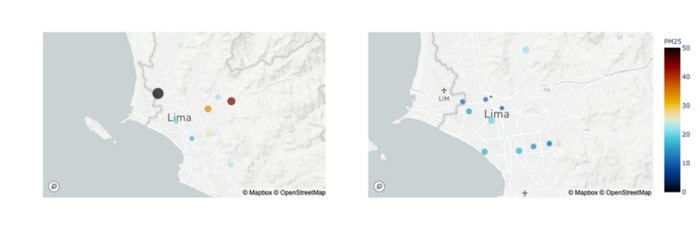
\includegraphics[width=.8\textwidth]{limamap.png}
    \caption{Ground-level air quality comparison in Lima, Peru: PM2.5 levels before (left) and after COVID19 (right) lockdown. Sources: QAIRA (Unicef Venture Fund), PlumeLab, OpenAQ.}
    \label{fig:limamap}
\end{figure*}

\begin{figure}[t]
    \centering
    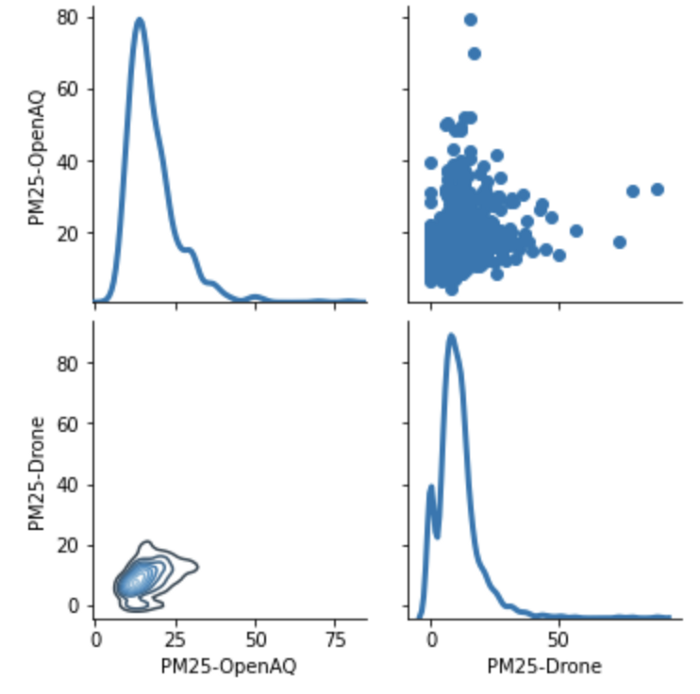
\includegraphics[width=.8\linewidth]{pmsummary.png}
    \caption{Comparison of PM2.5 readings from two different sources: Remote Sensing (OpenAQ) and ground-level (Drone).}
    \label{fig:summary}
\end{figure}

In this article, we have introduced the problem of developing a global-level machine learning model of accurately predicting air quality — especially in the wake of COVID19 imposed lockdowns —with multiple operational objectives. The next article shall incorporate the bi-level satellite data and features extracted from the secondary data sources in Table~\ref{tab:datatable} into an XGBoost to model PM2.5 globally. These secondary data sources include additional features such as population density and 2020 Covid-19 lockdown data that are known to significantly affect ground-level PM2.5 concentrations \cite{Hale}.